\chapter{Introduction}

%Channel limit
%
%URC
%Deep fade
%drop out
%5G

For all types of communication an important aspect is the channel through which the message is transmitted, for wireless communication, this is even more the case. The transmission of the message can be done in different environments, which have different impacts on the received signal. Common for all the environments is they introduce fading, which if not accounted for can have devastating effects for the transmission. 

Fading occurs when multipath propagation is present, that will introduce points in space where the waves adds either constructively or destructively, as can be seen on \autoref{intro_fading}. The constructive spots is not of much interest as it is only a couple of dB's difference, however the destructive interference can create spots with losses that borders minus infinite dB's. These spots are called deep fades and is is where the communication might suffer a drop out. A drop out occurs if the transmitted signal drops below the RX sensitivity level so the signal is lost. There are different tools to heighten the chance for the RX to receive signals that drops low and therefore increase the reliability of the communication link


\begin{figure}[H]
\centering
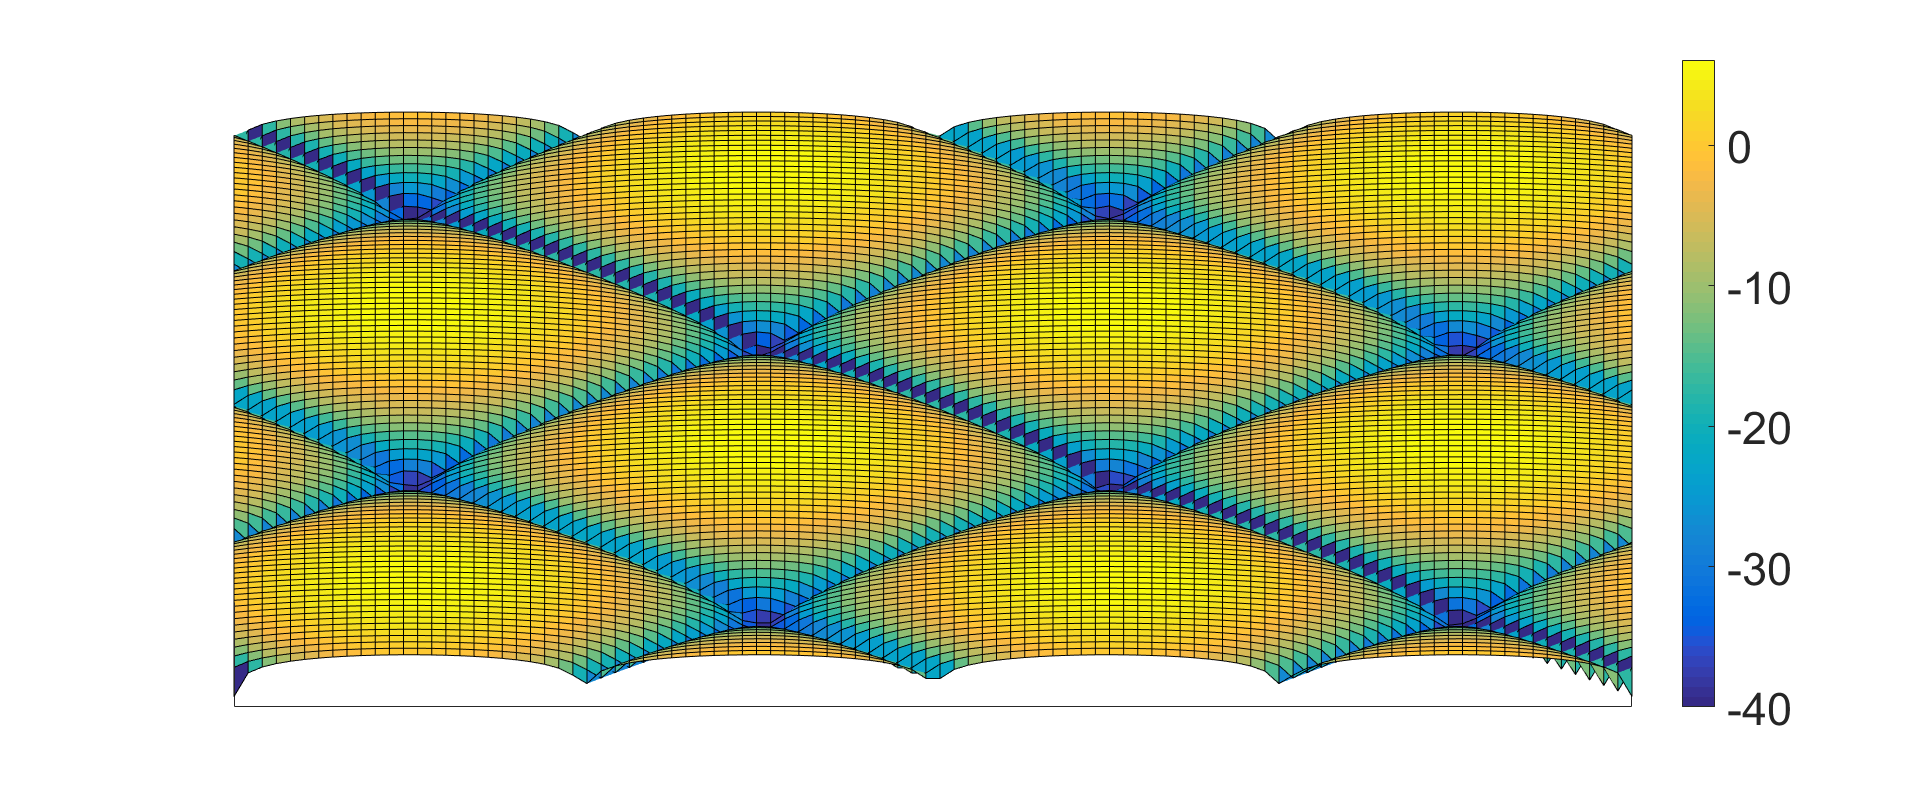
\includegraphics[width=\textwidth]{figures/intro_fading.png}
\caption{Fading gain from two wave fronts meeting, the deep fade spots have been elevated to allow for a better color resolution.}
\label{intro_fading}
\end{figure}

\section{Motivation}
With the development of the 5G wireless cellular network, a new concept have been introduced, \gls{URC}. \todo{source} Where earlier networks have run with a drop out probability of 0.1\% \todo{source}, with URC the drop out probability shall be under 0.001-0.0001\% \todo{source}. The reason to introduce this new feature is to accommodate special needs in critical systems \todo{source}. Today those systems use a wired channel which provide a higher reliability, but comes with a greater cost both price wise and installation wise, however new critical system is also predicted to need this feature in the future \todo{source}. %By having a better reliability, there is a higher chance that some new application can be used on the cellular network. 
Some of the applications needing a URC channel could be self driving cars, in emergency cases, is it not only necessary to provide low latency the certainty of the message to arrive is also desired. %where short message about position and speed can be send to other cars in the area, with low chance of needing re-transmission, which is importing in case of high alert situations. 
Other system that can gain advantages with URC, is systems where the communication window is very small and therefore do not have time for re-transmissions or a lot of data processing e.g. in error coding.


A problem about this is that to get this URC scenario, an in depth description of the channel is needed. A way to get higher reliability is to transmit with a higher power level, so there gets a higher \gls{SNR} on the communication link. But even if the overall signal is higher, there will still be problem with fading in some points in space. 


\begin{figure}[H]
\centering
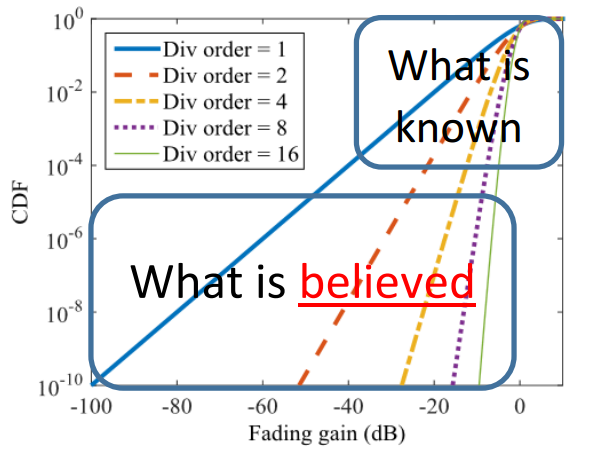
\includegraphics[width=0.65\textwidth]{figures/fading_gain.png}
\caption{\gls{CDF} of fading gain in different channel environments.}
\label{fading_gain}
\end{figure}


\section{Project outline}


%Ultra reliable communication (URC) is a concept, that will be introduced with the new 5G Wireless Systems. (Petar) It is one's of the new features that will come with the 5G network. The 4G network and 4G LTE network works with a block/bit error rate on $10^{-3}$, which is a very normal standard of error rate. But URC introduces a error rate on $10^{-5}$-$10^{-6}$. This of course comes with cost of either higher signal needed to be send, to get a higher signal-to-noise ratio (SNR) or lower bit rates, to introduce more error coding. But the return of this, a higher reliability and a lower latency is introduced. By having this two features introduced, more automatic and/or high precision machines can be connected to the network. An example is the use of the cellular network, to get self-driving cars to communicated with each other. In the case, that a car have to make a fast braking action, this have to be communicated to the cars behind it, with high reliability and low latency. So be introducing this URC, the cellular network can be used for more than just communication between humans, but also for fast and precises communication between machines.


